\section{Solución de Preguntas}
Ahora se procederá a responder todas las preguntas que se plantearón al inicio de la investigación.



\subsection{Caracter descriptivo}

%\begin{enumerate}
A continuación se enumeran los promedios de la variable total ploblación en cada uno de los años del DataSet:
%\item los promedios por  año de los ciudadanos en EEUU, son los siguientes\\
\begin{itemize}
\item promedio del año 1990:
[1] 79300.61

\item promedio del año 2000:
[1] 89735.04

\item promedio del año 2010:
[1] 98430.44

\item promedio del año 2011:
[1] 99337.63

\end{itemize}

%\item Ciudad con más población en 1990
% latex table generated in R 3.2.3 by xtable 1.8-2 package
% Wed Apr 06 07:34:08 2016
\begin{table}[ht]
\centering
\begin{tabular}{rllr}
  \hline
 & Ciudad & Estado & Poblacion \\ 
  \hline
1 & Los Angeles & California & 8863164 \\ 
   \hline
\end{tabular}
\caption{Ciudad con más población en el año 1990} 
\end{table}


%Ciudades con menos población en el año 1990
% latex table generated in R 3.2.3 by xtable 1.8-2 package
% Wed Apr 06 07:34:08 2016
\begin{table}[ht]
\centering
\begin{tabular}{rllr}
  \hline
 & Ciudad & Estado & Poblacion \\ 
  \hline
1 & Loving & Texas & 107 \\ 
   \hline
\end{tabular}
\caption{Ciudad con menos población en el año 1990} 
\end{table}


%\item Ciudad con más población en 2000
% latex table generated in R 3.2.3 by xtable 1.8-2 package
% Wed Apr 06 07:34:08 2016
\begin{table}[ht]
\centering
\begin{tabular}{rllr}
  \hline
 & Ciudad & Estado & Poblacion \\ 
  \hline
1 & Los Angeles & California & 8863164 \\ 
   \hline
\end{tabular}
\caption{Ciudad con más población en el año 2000} 
\end{table}


%Ciudades con menos población en el año 2000
% latex table generated in R 3.2.3 by xtable 1.8-2 package
% Wed Apr 06 07:34:08 2016
\begin{table}[ht]
\centering
\begin{tabular}{rllr}
  \hline
 & Ciudad & Estado & Poblacion \\ 
  \hline
1 & Loving & Texas &  67 \\ 
   \hline
\end{tabular}
\caption{Ciudad con menos población en el año 2000} 
\end{table}


%\item Ciudad con más población en 2010
% latex table generated in R 3.2.3 by xtable 1.8-2 package
% Wed Apr 06 07:34:08 2016
\begin{table}[ht]
\centering
\begin{tabular}{rllr}
  \hline
 & Ciudad & Estado & Poblacion \\ 
  \hline
1 & Los Angeles & California & 9818605 \\ 
   \hline
\end{tabular}
\caption{Ciudad con más población en el año 2010} 
\end{table}


%Ciudades con menos población en el año 2010
% latex table generated in R 3.2.3 by xtable 1.8-2 package
% Wed Apr 06 07:34:08 2016
\begin{table}[ht]
\centering
\begin{tabular}{rllr}
  \hline
 & Ciudad & Estado & Poblacion \\ 
  \hline
1 & Loving & Texas &  82 \\ 
   \hline
\end{tabular}
\caption{Ciudad con menos pobl. en 2010} 
\end{table}


%\item Ciudad con más población en 2011
% latex table generated in R 3.2.3 by xtable 1.8-2 package
% Wed Apr 06 07:34:08 2016
\begin{table}[ht]
\centering
\begin{tabular}{rllr}
  \hline
 & Ciudad & Estado & Poblacion \\ 
  \hline
1 & Los Angeles & California & 9889056 \\ 
   \hline
\end{tabular}
\caption{Ciudad con más población en el año 2011} 
\end{table}


%Ciudades con menos población en el año 2011
% latex table generated in R 3.2.3 by xtable 1.8-2 package
% Wed Apr 06 07:34:08 2016
\begin{table}[ht]
\centering
\begin{tabular}{rllr}
  \hline
 & Ciudad & Estado & Poblacion \\ 
  \hline
1 & Kalawao & Hawaii &  90 \\ 
   \hline
\end{tabular}
\caption{Ciudad con menos población en el año 2011} 
\end{table}


%A continuación se enumera las medias de la variables Total Población (TP), Total Población  No Hispana (TPNH) y Total Ploblación Hispana (TPH) en cada uno de los años del DataSet:
%\item los promedios por año de ciudadanos hispanos, son los siguientes\\
%\begin{itemize}
%\item promedio del año 1990:
%<<mseisa,results='asis',echo=FALSE, warning=FALSE, message=FALSE>>=
%	mean(datos1990$TPH)
%@
%\item promedio del año 2000:
%<<seisb,results='asis',echo=FALSE, warning=FALSE, message=FALSE>>=
%	mean(datos2000$TPH)
%@
%\item promedio del año 2010:
%<<seisc,results='asis',echo=FALSE, warning=FALSE, message=FALSE>>=
%	mean(datos2010$TPH)
%@
%\item promedio del año 2011:
%<<seisd,results='asis',echo=FALSE, warning=FALSE, message=FALSE>>=
%	mean(datos2011$TPH)
%@
%\end{itemize}
%	grupoMediaTP 	<- c(mean(datos1990$TP), mean(datos2000$TP), mean(datos2010$TP), mean(datos2011$TP))
%	grupoMediaTPNH 	<- c(mean(datos1990$TPNH), mean(datos2000$TPNH), mean(datos2010$TPNH),  mean(datos2011$TPNH))
%	grupoMediaTPH 	<- c(mean(datos1990$TPH), mean(datos2000$TPH), mean(datos2010$TPH), mean(datos2011$TPH))
%	mediasFull<-data.frame(TP=grupoMediaTP, TPNH=grupoMediaTPNH, TPH=grupoMediaTPH)	 	
%	xtable(mediasFull,"Valores de las medias en TP, TPHN y TPH")
A continuación se enumera las medias de la variables Total Población (TP), Total Población  No Hispana (TPNH) y Total Ploblación Hispana (TPH) en cada uno de los años del DataSet:

% latex table generated in R 3.2.3 by xtable 1.8-2 package
% Wed Apr 06 07:34:08 2016
\begin{table}[ht]
\centering
\begin{tabular}{rrrrr}
  \hline
 & Año 1990 & Año 2000 & Año 2010 & Año 2011 \\ 
  \hline
Media TP & 79300.61 & 89735.04 & 98430.44 & 99337.63 \\ 
  Media TPNH & 72172.49 & 78476.90 & 82336.35 & 82743.80 \\ 
  Media TPH & 7128.13 & 11258.14 & 16094.09 & 16593.83 \\ 
   \hline
\end{tabular}
\caption{Valores de las medias en TP, TPHN y TPH} 
\end{table}



El análisis continua con los siguientes resultados.
%Ciudad con mas población hispana en el año 1990
% latex table generated in R 3.2.3 by xtable 1.8-2 package
% Wed Apr 06 07:34:09 2016
\begin{table}[ht]
\centering
\begin{tabular}{rllr}
  \hline
 & Ciudad & Estado & PoblacionH \\ 
  \hline
1 & Los Angeles & California & 3351242 \\ 
   \hline
\end{tabular}
\caption{Ciudad con mayor TPH en el año 1990} 
\end{table}


%Ciudades con menos población hispana en el año 1990
% latex table generated in R 3.2.3 by xtable 1.8-2 package
% Wed Apr 06 07:34:09 2016
\begin{table}[ht]
\centering
\begin{tabular}{rllr}
  \hline
 & Ciudad & Estado & PoblacionH \\ 
  \hline
1 & Garfield & Montana &   0 \\ 
  2 & Petroleum & Montana &   0 \\ 
  3 & Arthur & Nebraska &   0 \\ 
  4 & Blaine & Nebraska &   0 \\ 
  5 & McPherson & Nebraska &   0 \\ 
  6 & Wheeler & Nebraska &   0 \\ 
  7 & Billings & North Dakota &   0 \\ 
  8 & Campbell & South Dakota &   0 \\ 
  9 & McPherson & South Dakota &   0 \\ 
   \hline
\end{tabular}
\caption{Ciudad con menor TPH en el año 1990} 
\end{table}


%Ciudad con más población hispana en el año 2000
% latex table generated in R 3.2.3 by xtable 1.8-2 package
% Wed Apr 06 07:34:09 2016
\begin{table}[ht]
\centering
\begin{tabular}{rllr}
  \hline
 & Ciudad & Estado & PoblacionH \\ 
  \hline
1 & Los Angeles & California & 4242213 \\ 
   \hline
\end{tabular}
\caption{Ciudad con mayor TPH en el año 2000} 
\end{table}


%Ciudades con menos población hispana en el año 2000
% latex table generated in R 3.2.3 by xtable 1.8-2 package
% Wed Apr 06 07:34:09 2016
\begin{table}[ht]
\centering
\begin{tabular}{rllr}
  \hline
 & Ciudad & Estado & PoblacionH \\ 
  \hline
1 & Blaine & Nebraska &   1 \\ 
  2 & Slope & North Dakota &   1 \\ 
   \hline
\end{tabular}
\caption{Ciudad con menor TPH en el año 2000} 
\end{table}


%Ciudad con más población hispana en el año 2010
% latex table generated in R 3.2.3 by xtable 1.8-2 package
% Wed Apr 06 07:34:09 2016
\begin{table}[ht]
\centering
\begin{tabular}{rllr}
  \hline
 & Ciudad & Estado & PoblacionH \\ 
  \hline
1 & Los Angeles & California & 4687889 \\ 
   \hline
\end{tabular}
\caption{Ciudad con mayor TPH en el año 2010} 
\end{table}


%Ciudad con menos población hispana en el año 2010
% latex table generated in R 3.2.3 by xtable 1.8-2 package
% Wed Apr 06 07:34:09 2016
\begin{table}[ht]
\centering
\begin{tabular}{rllr}
  \hline
 & Ciudad & Estado & PoblacionH \\ 
  \hline
1 & Blaine & Nebraska &   0 \\ 
   \hline
\end{tabular}
\caption{Ciudad con menor TPH en el año 2010} 
\end{table}


%Ciudad con más población hispana en el año 2011
% latex table generated in R 3.2.3 by xtable 1.8-2 package
% Wed Apr 06 07:34:09 2016
\begin{table}[ht]
\centering
\begin{tabular}{rllr}
  \hline
 & Ciudad & Estado & PoblacionH \\ 
  \hline
1 & Los Angeles & California & 4760974 \\ 
   \hline
\end{tabular}
\caption{Ciudad con mayor TPH en el año 2011} 
\end{table}


%Ciudad con menos población hispana en el año 2011
% latex table generated in R 3.2.3 by xtable 1.8-2 package
% Wed Apr 06 07:34:09 2016
\begin{table}[ht]
\centering
\begin{tabular}{rllr}
  \hline
 & Ciudad & Estado & PoblacionH \\ 
  \hline
1 & Blaine & Nebraska &   0 \\ 
   \hline
\end{tabular}
\caption{Ciudad con menor TPH en el año 2011} 
\end{table}


\subsection{Matriz de correlación}
A continuación se visualiza la matriz de correlación que existe entre la variables cuantitativas del conjunto de datos: 
%Ciudad con menos población hispana en el año 2011
% latex table generated in R 3.2.3 by xtable 1.8-2 package
% Wed Apr 06 07:34:09 2016
\begin{table}[ht]
\centering
\begin{tabular}{rrrrrr}
  \hline
 & TP & TPNH & TPH & PPH & AP \\ 
  \hline
TP & 1.00 & 0.97 & 0.87 & 0.17 & 0.03 \\ 
  TPNH & 0.97 & 1.00 & 0.73 & 0.12 & 0.02 \\ 
  TPH & 0.87 & 0.73 & 1.00 & 0.25 & 0.04 \\ 
  PPH & 0.17 & 0.12 & 0.25 & 1.00 & 0.13 \\ 
  AP & 0.03 & 0.02 & 0.04 & 0.13 & 1.00 \\ 
   \hline
\end{tabular}
\caption{Matrix de correlación} 
\end{table}

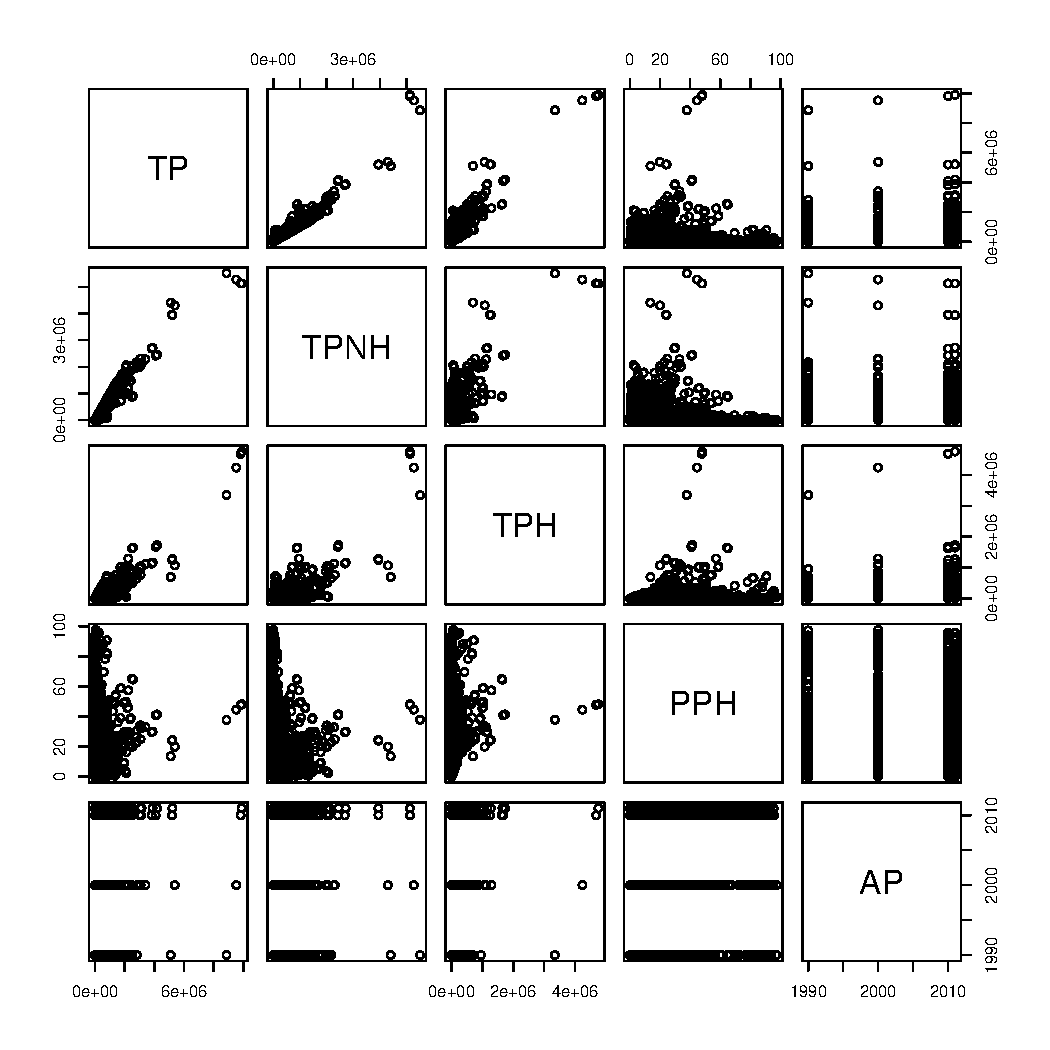
\includegraphics[width=\maxwidth]{figure/correlacion-1} 


